\subsection{Implementierung der Datenbank}
\label{subsec:implementierung-der-datenbank}

In diesem Unterkapitel werden die Einbindung der Datenbank in die Applikation sowie die Implementierung grob erläutert.
Der Hauptfokus liegt hierbei auf der Einbindung und der Methode zum Erstellen über Flask-SQLAlchemy.
Die Datenbank wurde mithilfe der Bibliothek Flask-SQLAlchemy erstellt.
Hierbei wurde die Bibliothek Flask-Migration für die Verwaltung von Datenbankschemata genutzt.

SQLAlchemy stellt \ac{ORM} bereit, mit welchem die relationalen Datenbanktabellen als objektorientierte Python-Klassen dargestellt werden können.
Dadurch konnte die in \ref{subsec:datenbankdesign-und-strukturkonzeption} dargestellte Datenbankstruktur, ohne die aktive Nutzung von SQL-Befehlen, definiert und umgesetzt werden.
Hierbei entspricht jede Klasse einer der Tabellen.
Die Attribute der Klassen bilden die Spalten der Tabellen ab. Die Fremdschlüssel zwischen den Tabellen werden über Relationship-Objekte beschrieben.
Die Klassen werden im Ordner \code{models} definiert.
Zur Veranschaulichung wird der Aufbau an dem Beispiel der Tabelle bzw. der Klasse \code{Report\_Table} aus der Datei \code{report.py} kurz erläutert, siehe Abbildung \ref{fig: Beispiel der Tabelle-Klasse Report-Table}.

\begin{figure}[H]
    \centering
    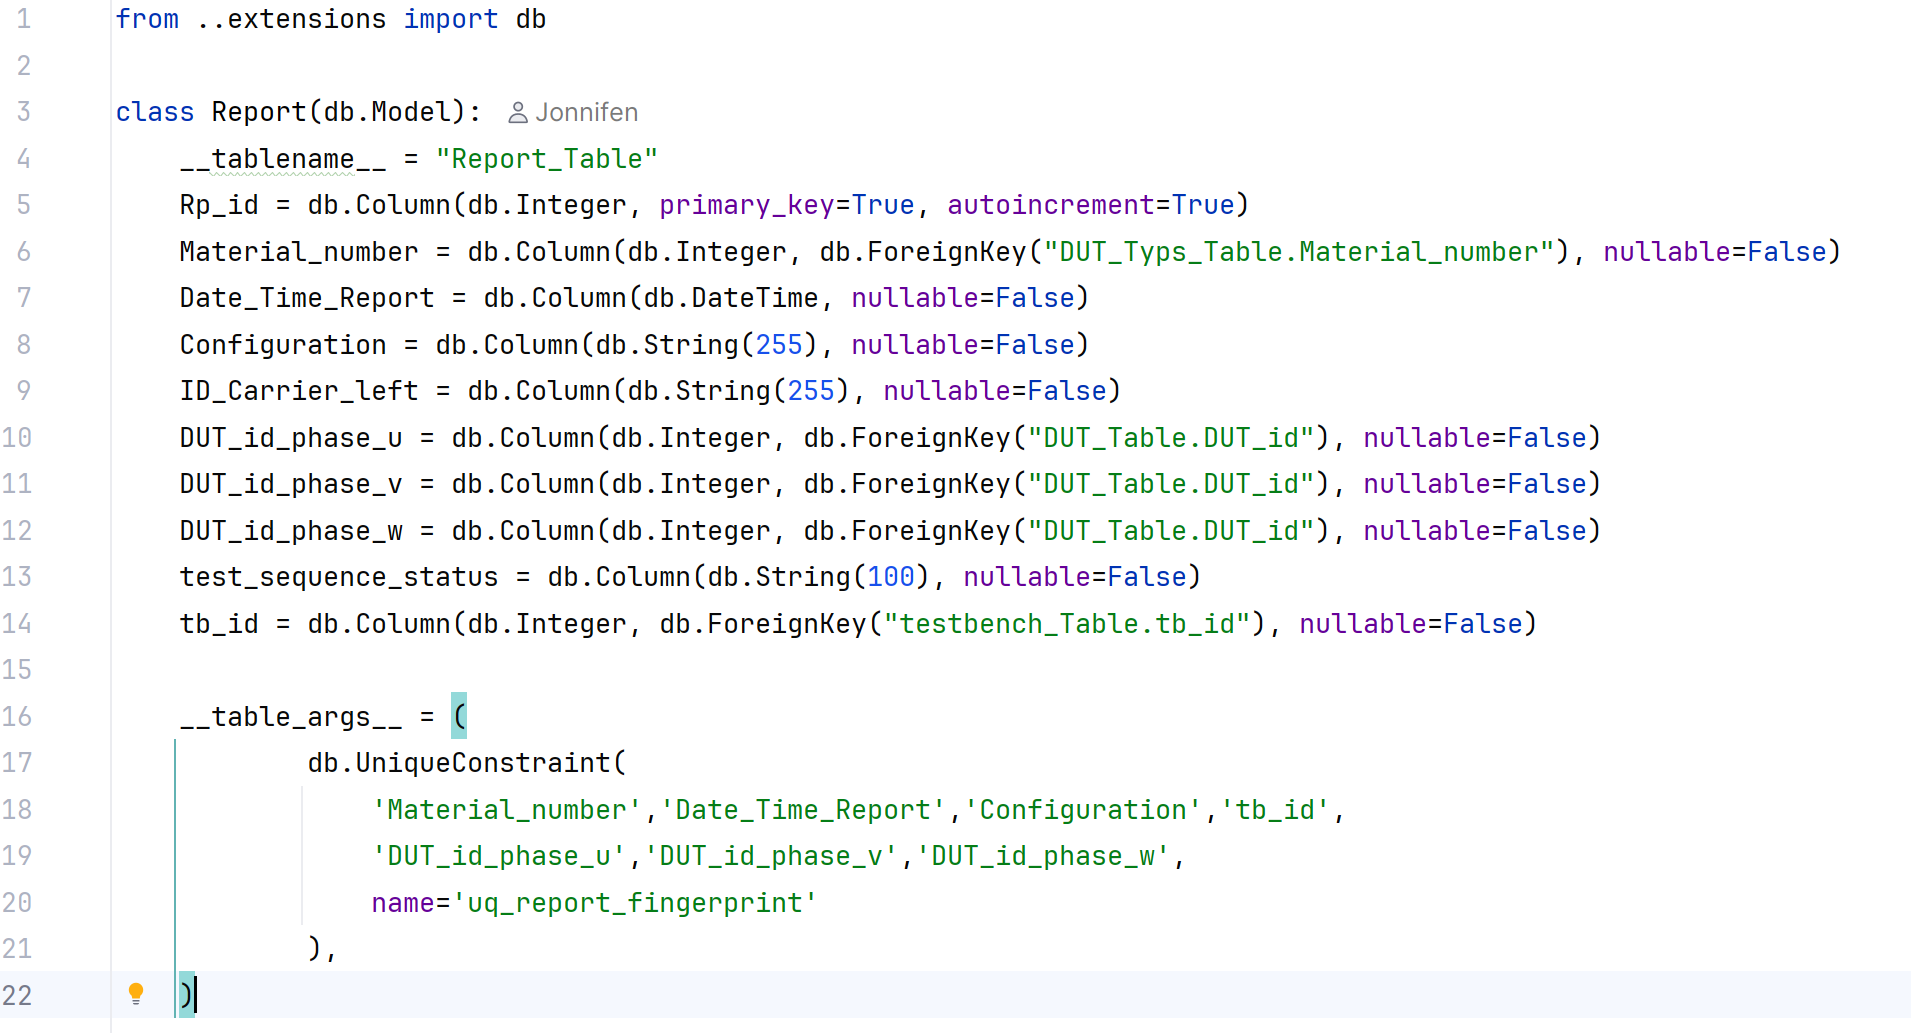
\includegraphics[width=1\textwidth]{Grafiken/5.4 Class.png}
    \caption{Beispiel der Tabelle-Klasse Report-Table}
    \label{fig: Beispiel der Tabelle-Klasse Report-Table}
    {Quelle: Eigene Darstellung}
\end{figure}



Alle Klassen aus \code{models} sind identisch aufgebaut und folgen demselben Schema.
Alle Klassen besitzen den Import der globalen Instanz \code{db} aus dem Modul \code{extensions}.
Diese Instanz bindet SQLAlchemy in die Flask-Applikation ein und wird beim Starten der Hauptapplikation initialisiert.
Über diese Instanz \code{db} können alle Modelle registriert und Datenbankoperationen wie Abfragen, Einfügungen oder Aktualisierungen ausgeführt werden.
Die Funktion zum Erstellen der Hauptapplikation ist in Abbildung \ref{fig: Funktion für das Erstellen der Hauptapplikation} abgebildet.
Sie liegt in der Datei \code{\_\_init\_\_.py} und wird über \code{run.py} ausgeführt.

\begin{figure}[H]
    \centering
    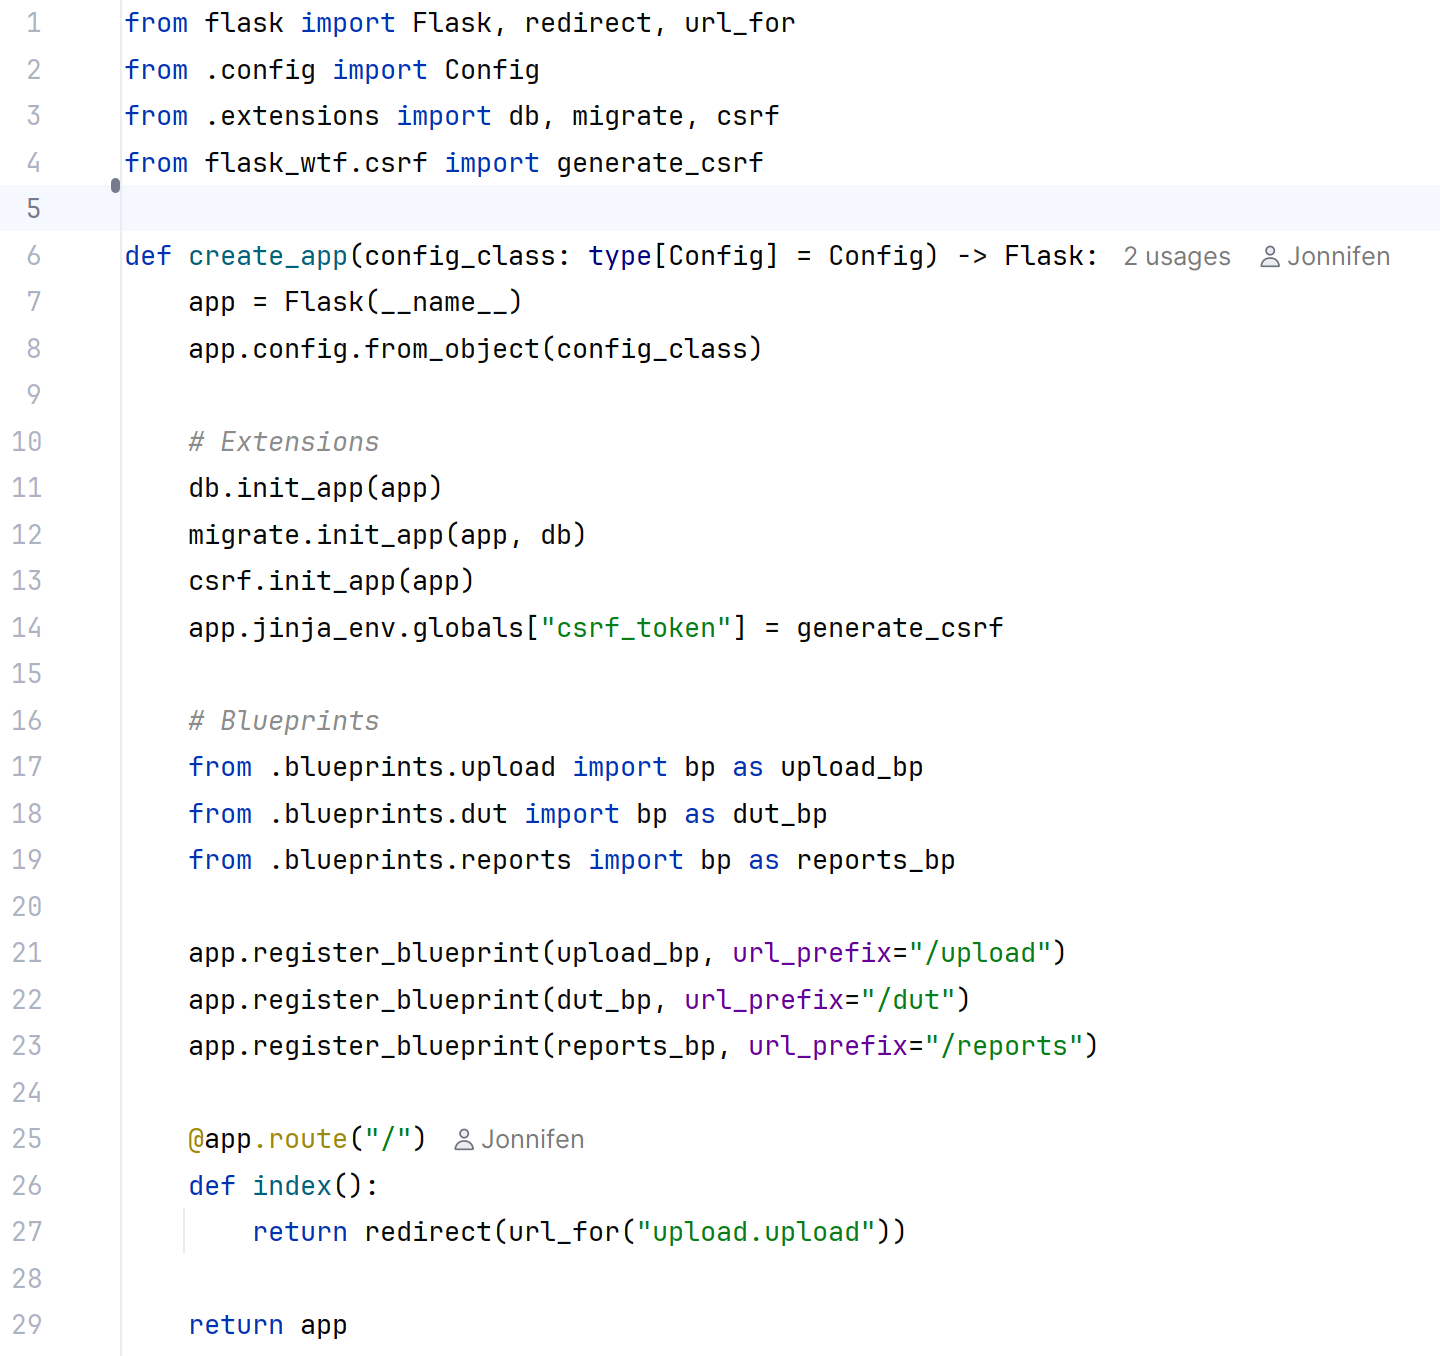
\includegraphics[width=1\textwidth]{Grafiken/createapp.png}
    \caption{Funktion für das Erstellen der Hauptapplikation}
    \label{fig: Funktion für das Erstellen der Hauptapplikation}
    {Quelle: Eigene Darstellung}
\end{figure}


Die Variable \code{\_\_tablename\_\_} in Abbildung \ref{fig: Beispiel der Tabelle-Klasse Report-Table} legt fest, wie die Tabelle in der Datenbank heißen soll.
In Zeile 5 bis 14 werden die Attribute bzw. die Tabellenspalte definiert.
Am Ende der Klasse wird ein Table-Constraint über \code{\_\_table\_args\_\_} definiert, welches als datenbankseitiger Duplizierungsschutz dient.
Dieser sorgt dafür, dass derselbe XML-Bericht versehentlich mehrfach importiert wird.
Es können nicht zwei Datensätze mit denselben Werten existieren.

Dies dient als zusätzliche Sicherheitsinstanz neben dem selbst erstellten Duplizierungsschutz in \code{ingest\_xml()}.
Die Verbindungen der Datenbank werden über die Klasse Config in der Datei \code{config.py} definiert.
Hierbei wird im Fall, dass die Datenbank nicht vorhanden ist und getestet werden soll, eine SQLite-Datenbank erstellt und genutzt.
Die genaue Bezeichnung der \code{DATENBANK\_URL} und dem \code{FLASK\_SECRET\_KEY} ist in \code{.env} definiert.
In der folgenden Abbildung \ref{fig:Config-Klasse für Datenbankverbindung} ist die Klasse \code{Config} zum Verbinden mit der Datenbank abgebildet.

\begin{figure}[H]
    \centering
    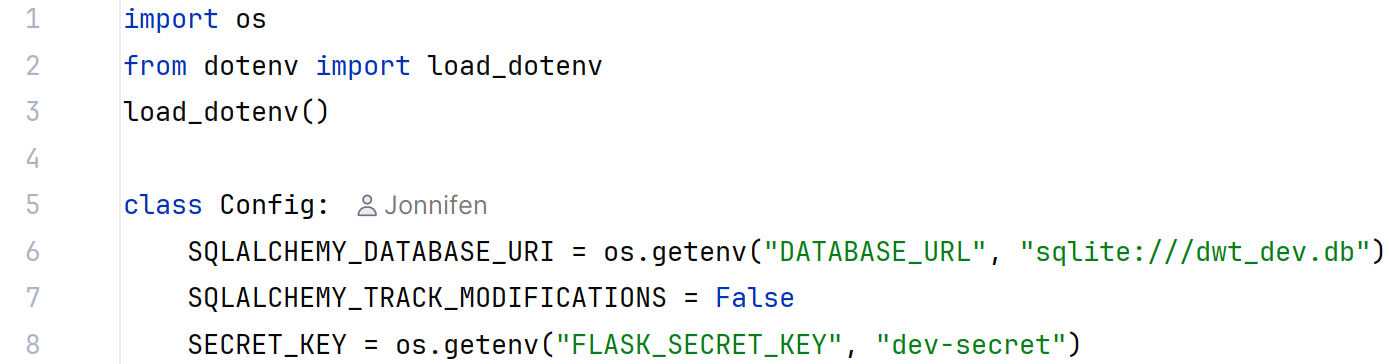
\includegraphics[width=1\textwidth]{Grafiken/Config.png}
    \caption{Config-Klasse für Datenbankverbindung}
    \label{fig:Config-Klasse für Datenbankverbindung}
    {Quelle: Eigene Darstellung}
\end{figure}

Zur Verwaltung und Versionierung des Datenbankschemas wird Flask-Migrate eingesetzt, welches auf dem Migrationstool Alembic basiert.
Diese Erweiterung erkennt automatisch Änderungen an den ORM-Modellen und erzeugt daraus sogenannte Migrationsskripte. Die Skripte sind im Ordner \code{versions} unter \code{migrations} zu finden.
Diese Skripte enthalten die notwendigen SQL-Befehle, um das Schema der Datenbank an Modellversionen anzupassen.
Durch die Befehle werden die Migrationen generiert und auf die bestehende Datenbank angewendet.
Dadurch ist es möglich, die Struktur der Datenbank schrittweise zu erweitern oder zu verändern, ohne bestehende Daten zu verlieren.
Diese Methode wurde hauptsächlich für die einfachere Entwicklung implementiert und wird nicht zwangsläufig in zukünftigen Versionen weiterverwendet.






